\chapter{Projekt systemu i elementy implementacji}
W~tym rozdziale zaprojektuję oprogramowanie realizujące cele opisane w~punkcie~\ref{lib-requirements}.
Zaproponuję sposób realizacji, możliwości i~ograniczenia poszczególnych jego elementów. Dla części komponentów stworzę prototypy.

\section{Specyfikacja wymagań systemowych (SWS)}
Z~celów tej pracy zawartych w~punkcie~\ref{lib-requirements} stworzyłem standardową listę konkretnych wymagań dla zespołu wytwórczego, czyli mnie samego.
Organizując niniejszą sekcję wzorowałem się na specyfikacji wymagań systemowych opisanej w~prezentacji ,,Inżynieria Wymagań'' Jarosława Kuchty, z~przedmiotu ,,Dokumentacja i~Jakość Oprogramowania''~\cite{kuchta}.


\subsection{Wstęp i~opis informacyjny}
Jako rozbudowana sekcja wstępu SWS służyły poprzednie rozdziały niniejszej pracy.
,,Szczegółowy opis problemów do rozwiązania'' znajduje się w~punkcie~\ref{lib-requirements}.


\subsubsection{Diagram przepływu najwyższego poziomu}
Diagram~\ref{fig:project-overview} przedstawia ogólne działanie systemu w~trakcie wywoływania zdalnej metody. Jest to główna funkcja mojego projektu. Funkcja drugorzędna -- tłumaczenie danych, również została ujęta.


Widoczny na schemacie klient jest jednym z~wielu, które mogą być stworzone przez kod korzystający z~mojej biblioteki.
Obiekt każdego klienta spełnia jakiś zadany interfejs. Robi to przez opakowywanie parametrów, zaadresowanie ich, wysłanie do obiektu faktycznie wykonującego kod i~odebranie wyniku.
Interfejs klienta i obiektu zdalnego są zgodne, chodź napisane w~różnych językach na różne platformy. Aby zminimalizować nakład pracy programisty, najlepiej byłoby, gdyby interfejs po stronie klienta (.NET) był generowany z~wersji serwerowej (Java, Android).
Tak samo jak w~przypadku interfejsów wygląda sprawa klas przekazywanych do metod jako parametry -- także muszą być zgodne, najlepiej automatycznie tłumaczone.
Typy przetłumaczone na schemacie oznaczone są apostrofem.
Kod kliencki nie musi zawierać tłumaczenia implementacji zdalnych interfejsów.
Współdzielone definicje klas danych i~interfejsów są niezbędne, aby uzyskać polimorfizm metod zdalnych.

Serwer jest tworzony przez kod kliencki i~nasłuchuje na żądania na zadanym interfejsie sieciowym. Może to być dowolna technologia pozwalająca na dwustronne wysyłanie wiadomości, np.\ TCP, HTTP, SSL/TLS, czy też strumienie w~pamięci (rozwiązanie lokalne).
Na schemacie serwer posiada tylko jeden obiekt zdalny klasy \texttt{Implementacja A}, ale faktycznie może posiadać ich wiele.

\begin{figure}
  \advance\leftskip-1.5cm
	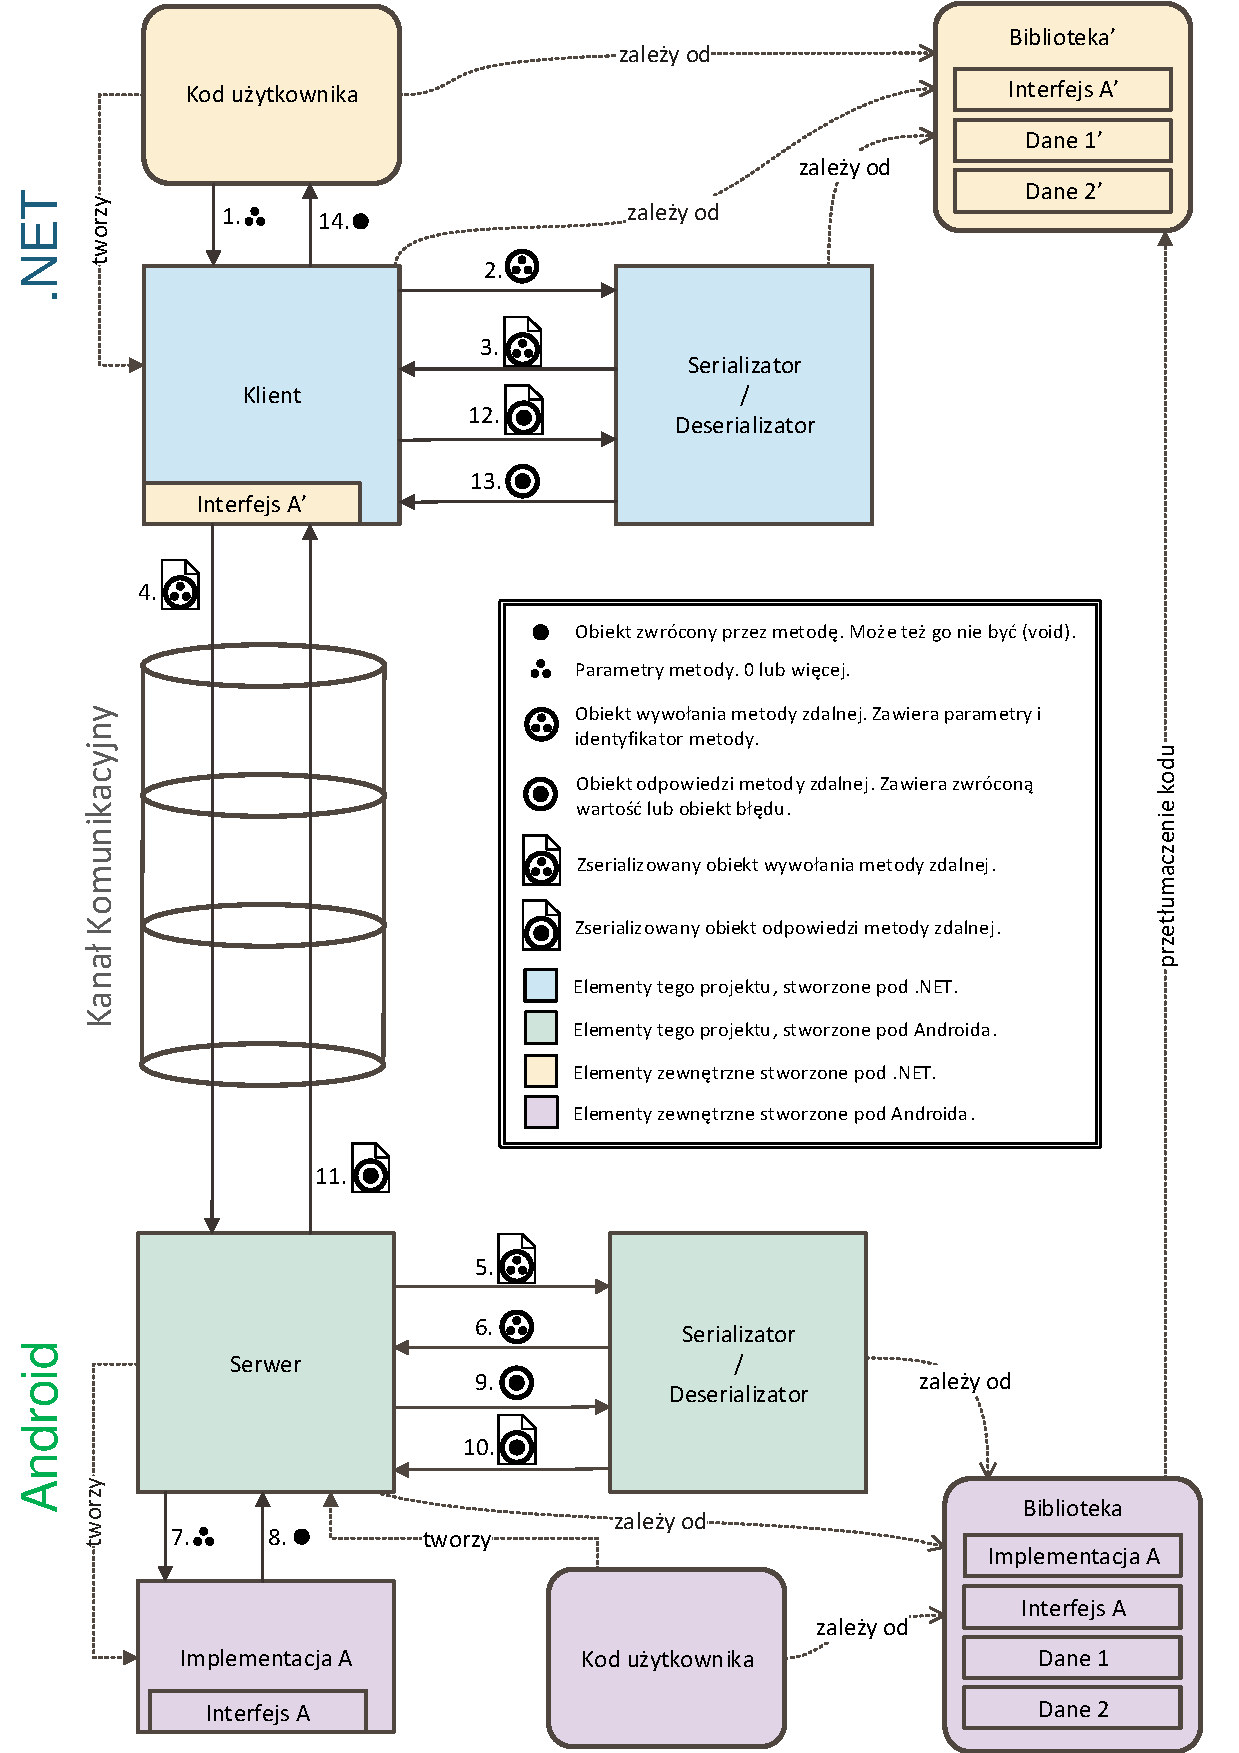
\includegraphics[scale=0.8]{img/schematy/schemat-dzialania-magisterki.pdf}
	\caption{Ogólny schemat projektu.}
	\label{fig:project-overview}
\end{figure}


\subsubsection{Reprezentacja zawartości informacyjnej}
Nie można właściwie mówić o~zawartości informacyjnej systemu, ponieważ takiej nie będzie.
Przez mój system dane będą jedynie przepływać.


\subsubsection{Opis interfejsów systemowych}
\begin{itemize}
	\item Jako, że to, co tworzę będzie kolekcją bibliotek Javy i~C\# będą one mogły być ładowane, a~ich klasy wykorzystywane przez zewnętrzne aplikacje.
	\item Niezależne narzędzie do generacji kodu będzie opatrzone w~interfejs linii poleceń.
\end{itemize}


\subsection{Wymagania funkcjonalne}
% WYMAGANIA POMIJANE:
% reliable sessions (w sumie też by mi się przydał jakiś mechanizm, który umożliwi komunikację w niestabilnym środowisku Internetu)
% \url{http://blogs.msdn.com/b/shycohen/archive/2006/02/20/535717.aspx} \\

\subsubsection{Ogólne}

\begin{description}
\itemtitle{Serializacja danych z zachowaniem informacji o typach}
Zserializowane reprezentacje obiektów muszą zawierać informacje o~typach wtedy, kiedy nie wynika ona jednoznacznie z~kontekstu,
np.\ przy zwracaniu ze zdalnej metody obiektu klasy dziedziczącej po tym, zdeklarowanym w~interfejsie tejże metody.
To wymaganie dotyczy zarówno strony klienta jak i~serwera.
Deserializacja powinna być komplementarna i~ze stworzonych reprezentacji odtwarzać obiekty o~odpowiednich typach i~z~poprawnymi danymi.
Taka metoda serializacji i~deserializacji jest warunkiem działania polimorficznych metod.

%\itemtitle{Tłumaczenie kodu}
%Zrealizowane jako niezależne narzędzie.
%Tłumaczenie kodu zmniejszyłoby nakład pracy programisty, który bez tego musiałby sam stworzyć odpowiadające klasy danych w~obu językach.
%Klasy i~pola nie znajdujące odpowiednika są pomijane w~trakcie tłumaczenia.
%Tłumaczenie powinno się odbywać z~Javy do C\#, ponieważ w~Javie będzie więcej kodu (kod implementacji zdalnych metod).
%Jeśli w danej klasie są inne klasy z zewnętrznej biblioteki, to trzeba też przetłumaczyć te. Trzeba dostarczyć kod wszystkich.
%Jeśli jedno ogniwo jest nieprzetłumaczalne to można pominąć pole z ostrzeżeniem.
\end{description}

\subsubsection{Serwer}

\begin{description}

\itemtitle{Komunikacja z~klientem}
Serwer powinien nasłuchiwać żądań od klientów na zadanym dwustronnym kanale komunikacyjnym.
Konkretny typ kanału (TCP, SSL, HTTP, itp.) nie jest ważny.
Może przyjmować wywołania metod i~przekierowywać je do obiektów zdalnych (względem klienta).
Przekazuje do klientów zwracane wartości.

\itemtitle{Wystawianie metod publicznych zadanych obiektów ,,na zewnątrz''}
Kod serwera ma przyjmować dowolny obiekt i~umożliwiać zdalnym klientom wywoływanie jego publicznych metod.
Parametry tych metod muszą być przetłumaczalne na kod klienta.

% Można się też zastanowić nad singletonami.
\itemtitle{Tworzenie zdalnych obiektów na życzenie klienta}
Po otrzymaniu specjalnego żądania kod serwera powinien stworzyć obiekt implementujący zadany interfejs i~zwrócić jego identyfikator. Klient będzie mógł wywoływać zdalnie metody na stworzonym obiekcie.

\itemtitle{Niszczenie zdalnych obiektów na życzenie klienta}
Specjalne żądanie zawierające identyfikator obiektu powinno powodować jego zwolnienie i~uniemożliwienie z~nim dalszej komunikacji.

\itemtitle{Polimorfizm parametrów metod zdalnych}
Metody zdalne muszą obsługiwać parametry wszystkich typów zgodnych ze spodziewanym. Dla przykładu, metoda przyjmuje parametr typu A, więc powinna przyjąć też parametry wszystkich typów dziedziczących po A.

\itemtitle{Przeciążanie metod zdalnych}
Metody zdalne mogą być przeciążane, tj.\ dwie metody mogą mieć tę samą nazwę, ale inny zestaw parametrów.

\itemtitle{Komunikacja z systemem Android}
Obiekty zdalne muszą mieć możliwość wywoływania metod z~API Androida.

\end{description}

\subsubsection{Klient}

\begin{description}

\itemtitle{Tworzenie obiektów klienckich}
Biblioteka po stronie .NET musi być w~stanie dynamicznie stworzyć obiekt klienta dla obiektu zdalnego.
Każdy klient spełnia jakiś zadany interfejs.

\itemtitle{Nawiązywanie sesji z~serwerem}
Obiekt klienta nawiązuje kontakt z~serwerem poprzez dowolny dwustronny kanał komunikacyjny (na którym serwer nasłuchuje).
Następnie żąda od serwera stworzenia dla siebie zdalnego obiektu.
Wszystkie metody z~interfejsu zdalnego wywoływane na kliencie są przekazywane do jednego obiektu zdalnego.
Zwolnienie obiektu klienta powoduje zwolnienie obiektu zdalnego.

\itemtitle{Konsumowanie polimorficznych metod zdalnych}
Klient wykonuje metody implementowanego przez siebie interfejsu przez delegację (i~wysłanie) ich do obiektu zdalnego.
Wysłanie poprzedzane jest serializacją, podczas której muszą zostać zachowane informacje o~typach parametrów oraz ich ewentualnych obiektach składowych.

\end{description}


\subsection{Wymagania niefunkcjonalne}

\begin{description}

\itemtitle{Serwer na Androidzie}
Kod serwera musi działać na platformie Android.

\itemtitle{Klient w~.NET pod Windows}
Kod klienta musi działać na platformie .NET\@.

\itemtitle{Wydajność serwera}
Nie musi być duża, jako, że nie jest priorytetem projektu. Wystarczy jednoczesna obsługa pięciu (5) klientów.

\itemtitle{Rozszerzalność metod zdalnych bez ingerencji w oryginalny kod}
Funkcjonalność metod zdalnych powinna być rozszerzalna bez ingerencji w~ich kod dzięki mechanizmom programowania obiektowego.
Przykładem jest możliwość przyjmowania przez metodę zdalną obiektu klasy dziedziczącej po spodziewanym typie parametru, bez potrzeby jakiejkolwiek ingerencji w~kod metody, aby mogła rozumieć nową klasę.
Jednak definicja nowej klasy musi być dostępna zarówno dla klienta, jak i~serwera.

\itemtitle{Łatwość użytkowania}
Budowanie i~korzystanie z~bibliotek, które powstaną w~trakcie realizacji tego projektu, powinno być proste i~intuicyjne.

\end{description}



\section{Używana konfiguracja sprzętowa i~narzędzia}
\label{system-configuration}
Przed przystąpieniem do omawiania komponentów rozwiązania warto wspomnieć o~tym, na jakiej konfiguracji sprzętowej oraz za pomocą jakich narzędzi były wytwarzane kod i~tekst niniejszej pracy. Na tej samej konfiguracji wykonywane były testy \emph{frameworków} w~rozdziale~\ref{similar-technologies}.

\begin{description}
\itemtitle{System operacyjny}
Windows 7 Professional x64. Cały kod i~tekst pracy powstał na tej maszynie. Na niej był też osadzony emulator Androida.

\itemtitle{Emulator Androida}
Ściągnięty razem z~IDE Eclipse zmodyfikowanym do pracy z~Androidem\footnote{Do ściągnięcia ze strony \url{http://developer.android.com/sdk/index.html}}.
Jest to standardowy emulator od Google\footnote{Alternatywnym emulatorem jest Genymotion (\url{http://www.genymotion.com/}), polecany na stronach Xamarina.}.
Emulowany był Android 4.4.2 (poziom API Androida w~tej wersji to 19). Reszta konfiguracji emulowanego urządzenia: typ obrazu~-- \emph{ARM EABI v7a}, urządzenie~-- Nexus S, RAM~-- 512MB, \emph{VM Heap}~-- 32MB, wewnętrzna pamięć~-- 200MB, karta SD~-- 50MB, zaznaczona opcja użycia GPU hosta.
%Używam ARMowego, bo więcej telefonów jest właśnie na nim. Zdażają się też drobne rozbieżności działania niektórych niskopoziomowych aplikacji względem obrazu na architekturę x86 (\emph{Intel x86 Atom}).

\itemtitle{Eclipse 4.2.1 z~wtyczką ADT}
Przy jego użyciu stworzona jest przykładowa aplikacja serwerowa, a~także inne aplikacje powstające w~trakcie testów \emph{frameworków} (rozdział~\ref{similar-technologies}). ADT -- \emph{Android Development Tools}, to wtyczka umożliwiająca tworzenie kodu na Androida.

\itemtitle{NetBeans 7.4}
Kod Javy niewymagający Androida do działania powstawał w~nim.

\itemtitle{Visual Studio 2013 Ultimate}
Pod nim powstawał cały kod C\#.

\itemtitle{Tortoise GIT}
GIT jest systemem kontroli wersji w~którym trzymany jest kod oraz tekst tej pracy. Wykorzystywany przeze mnie klient to TortoiseGit\footnote{Do pobrania ze strony \url{https://code.google.com/p/tortoisegit/}}. Repozytorium znajduje się pod adresem \url{https://github.com/butla/SimRemo}.

\itemtitle{\LaTeX}
Tekst pracy pisany jest z~użyciem technologii \LaTeX. Jako edytor wykorzystywany jest program TeXnicCenter\footnote{\url{http://www.texniccenter.org/}}.
\end{description}

%Do testów wymagane jest przekierowanie portu TCP hosta do portu TCP emulatora. Do tego należy użyć komendy:
%\begin{lstlisting}[language=bash]
%adb forward tcp:1666 tcp:1666
%\end{lstlisting}
%Adb to komenda z narzędzi instalowanych z Eclipsem.



\section{Częściowa implementacja}
Tutaj przedstawię zaimplementowaną część zaplanowanego projektu. Całość okazała się zbyt obszerna na jedną pracę dyplomową. W~dalszej części rozdziału dokładniej przedstawię poszczególne elementy systemu (zarówno te zaimplementowane jak i~nie) oraz wyzwania z~nimi związane. Uzasadnię też metody ich implementacji.

\subsection{Spełnienie wymagań systemowych}
Spełnienie zdefiniowanych wymagań systemowych przez stworzoną implementację zostało przedstawione w~tabeli~\ref{tab:requirements-fulfilment}.

\begin{table}[htbp]
	  \caption[Spełnienie wymagań systemowych.]{Spełnienie wymagań systemowych. ,,+'' oznacza, że wymaganie jest spełnione; ,,+\textasciitilde'', że zostało spełnione ale wymaga komentarza; ,,--'' że nie zostało spełnione.}
	\begin{adjustbox}{center}
		\begin{tabular}{ @{}| c | c | c | c | }
			\hline
				\textbf{Nazwa wymagania} & \textbf{Typ wymagania} & \textbf{Obszar} & \textbf{Wykonanie}\\
				\hline \hline
				Serializacja danych z zachowaniem informacji o typach & Funkcjonalne & Ogólne & +\textasciitilde\\
				\hline
				
				Komunikacja z~klientem & Funkcjonalne & Serwer & +\\
				\hline
				Wystawianie metod publicznych zadanych obiektów ,,na zewnątrz'' & Funkcjonalne & Serwer & + \\
				\hline
				Tworzenie zdalnych obiektów na życzenie klienta & Funkcjonalne & Serwer & -- \\
				\hline
				Niszczenie zdalnych obiektów na życzenie klienta & Funkcjonalne & Serwer & -- \\
				\hline
				Polimorfizm parametrów metod zdalnych & Funkcjonalne & Serwer & + \\
				\hline
				Przeciążanie metod zdalnych & Funkcjonalne & Serwer & + \\
				\hline
				Komunikacja z systemem Android & Funkcjonalne & Serwer & + \\
				\hline
				
				Tworzenie obiektów klienckich & Funkcjonalne & Klient & +\textasciitilde \\
				\hline
				Nawiązywanie sesji z serwerem & Funkcjonalne & Klient & -- \\
				\hline
				Konsumowanie polimorficznych metod zdalnych & Funkcjonalne & Klient & + \\
				\hline
				
				Łatwość użytkowania & Niefunkcjonalne & Ogólne & +\textasciitilde \\
				\hline
				Serwer na Androidzie & Niefunkcjonalne & Serwer & + \\
				\hline
				Rozszerzalność metod zdalnych bez ingerencji w oryginalny kod & Niefunkcjonalne & Serwer & + \\
				\hline
				Wydajność serwera & Niefunkcjonalne & Serwer & + \\
				\hline
				Klient w .NET pod Windows & Niefunkcjonalne & Klient & + \\
				\hline
		\end{tabular}
	\end{adjustbox}
	\label{tab:requirements-fulfilment}
\end{table}

Komentarz do niespełnionych wymagań:
\begin{description}
\itemtitle{Tworzenie zdalnych obiektów na życzenie klienta}
Mechanizm w~ogóle nie zaimplementowany. Zdalne obiekty (serwisy) działają jako singletony; każdy obiekt musi być stworzony przez serwer i~powiązany z~unikatowym adresem. Wszystkie żądania wysłane na jeden adres są obsługiwane przez jedną instancję serwisu.

\itemtitle{Niszczenie zdalnych obiektów na życzenie klienta}
Ponieważ nie zostało zaimplementowane tworzenie obiektów na życzenie nie ma sensu implementować usuwania.

\itemtitle{Nawiązywanie sesji z serwerem}
Sesje miały być nawiązywane na zasadzie przyznawania każdemu klientowi osobnej instancji serwisu. Ponieważ klient nie może stworzyć obiektu zdalnego na serwerze to sesje nie mogą być zaimplementowane.
\end{description}

Są jeszcze wymagania zaimplementowane, które jednak wymagają komentarza:
\begin{description}
\itemtitle{Serializacja danych z zachowaniem informacji o typach}
Nie ma wsparcia dla oznaczania typów kolekcji: tablic, list, słowników itp.
\itemtitle{Tworzenie obiektów klienckich}
Kiedy zdalna metoda rzuci wyjątek, to pewien wyjątek jest rzucany przez metodę obiektu klienckiego. Nie jest to jednak przetłumaczony obiekt wyjątku rzuconego po stronie serwera, a~wyjątek typu \texttt{JsonRpcException} zawierający tekstowy zapis tego oryginalnego.

\itemtitle{Łatwość użytkowania}
Ustawianie słownika typów mogłoby się odbywać za pośrednictwem pliku konfiguracyjnego. Aktualnie odbywa się w~kodzie, za pomocą wywołania statycznej metody, która może być trudna do znalezienia, jeśli się nie wie gdzie szukać.
\end{description}


\subsection{Zasady działania}
Możliwości zaimplementowanego systemu to:
\begin{itemize}
	\item serwowanie publicznych metod wybranych obiektów zdalnie, z~Androida;
	\item dynamiczne tworzenie obiektów klienckich z~poziomu .NET; obiekty implementują zadany (zdalny) interfejs;
	\item polimorfizm parametrów metod zdalnych, ale tylko jeśli są pojedynczymi obiektami, a~nie kolekcjami;
	\item przeładowywanie metod zdalnych.
\end{itemize}

W~ogólności system pozwala na wystawienie publicznych metod zwykłego javowego obiektu ,,na zewnątrz'' systemu Android.
Taki wystawiany obiekt zwany jest od teraz obiektem zdalnym.
Program na Androidzie wystawiający obiekty zdalne działa jako serwer, konkretnie serwer JSON-RPC -- standardu zdalnego wywoływania metod opartego o~JSON, opisanego w~punkcie~\ref{json-rpc}.

System zawiera też klienta JSON-RPC pod .NET. Za jego pomocą można dynamicznie, wywołaniem jednej metody, stworzyć obiekt spełniający zadany interfejs będący klientem obiektu zdalnego.
Dla przykładu: kod na Androida zawiera interfejs \texttt{TestService} i~klasę \texttt{TestServiceImpl} go implementującą, obie stworzone przez hipotetycznego użytkownika mojego systemu, a~nie będące jego częścią.
Po stronie .NET musi znajdować się interfejs lustrzany dla \texttt{TestService} z~Javy (Androida), czyli posiadający tak samo nazwane metody z~analogicznymi parametrami.
Na bazie tego interfejsu tworzony jest obiekt kliencki dla obiektu zdalnego. Można na nim wykonywać metody interfejsu \texttt{TestService} tak jak na zwykłym lokalnym obiekcie -- zwracane wartości będą normalnymi obiektami.

Struktura tego, co zostało zaimplementowane przedstawiona jest na rysunku~\ref{fig:implementation-overview}.
Dokładniejsza struktura przygotowanej biblioteki .NET przedstawiona jest na rysunku~\ref{fig:dot-net-classes}.
Przygotowana przeze mnie część Androidowa to jedna klasa -- JsonRpcBasicServer -- dodana do jsonrpc4j\footnote{jsonrpc4j opisane w~punkcie~\ref{jsonrpc4j}.}. Więcej o~tym w~punkcie~\ref{android-rpc}.
Natomiast schemat działania zaimplementowanego systemu można zobaczyć na rysunku~\ref{fig:sequence-diagram}.
Ostatni diagram zawiera cztery sekwencje: A, B, C i D.
\begin{figure}
	\centering
		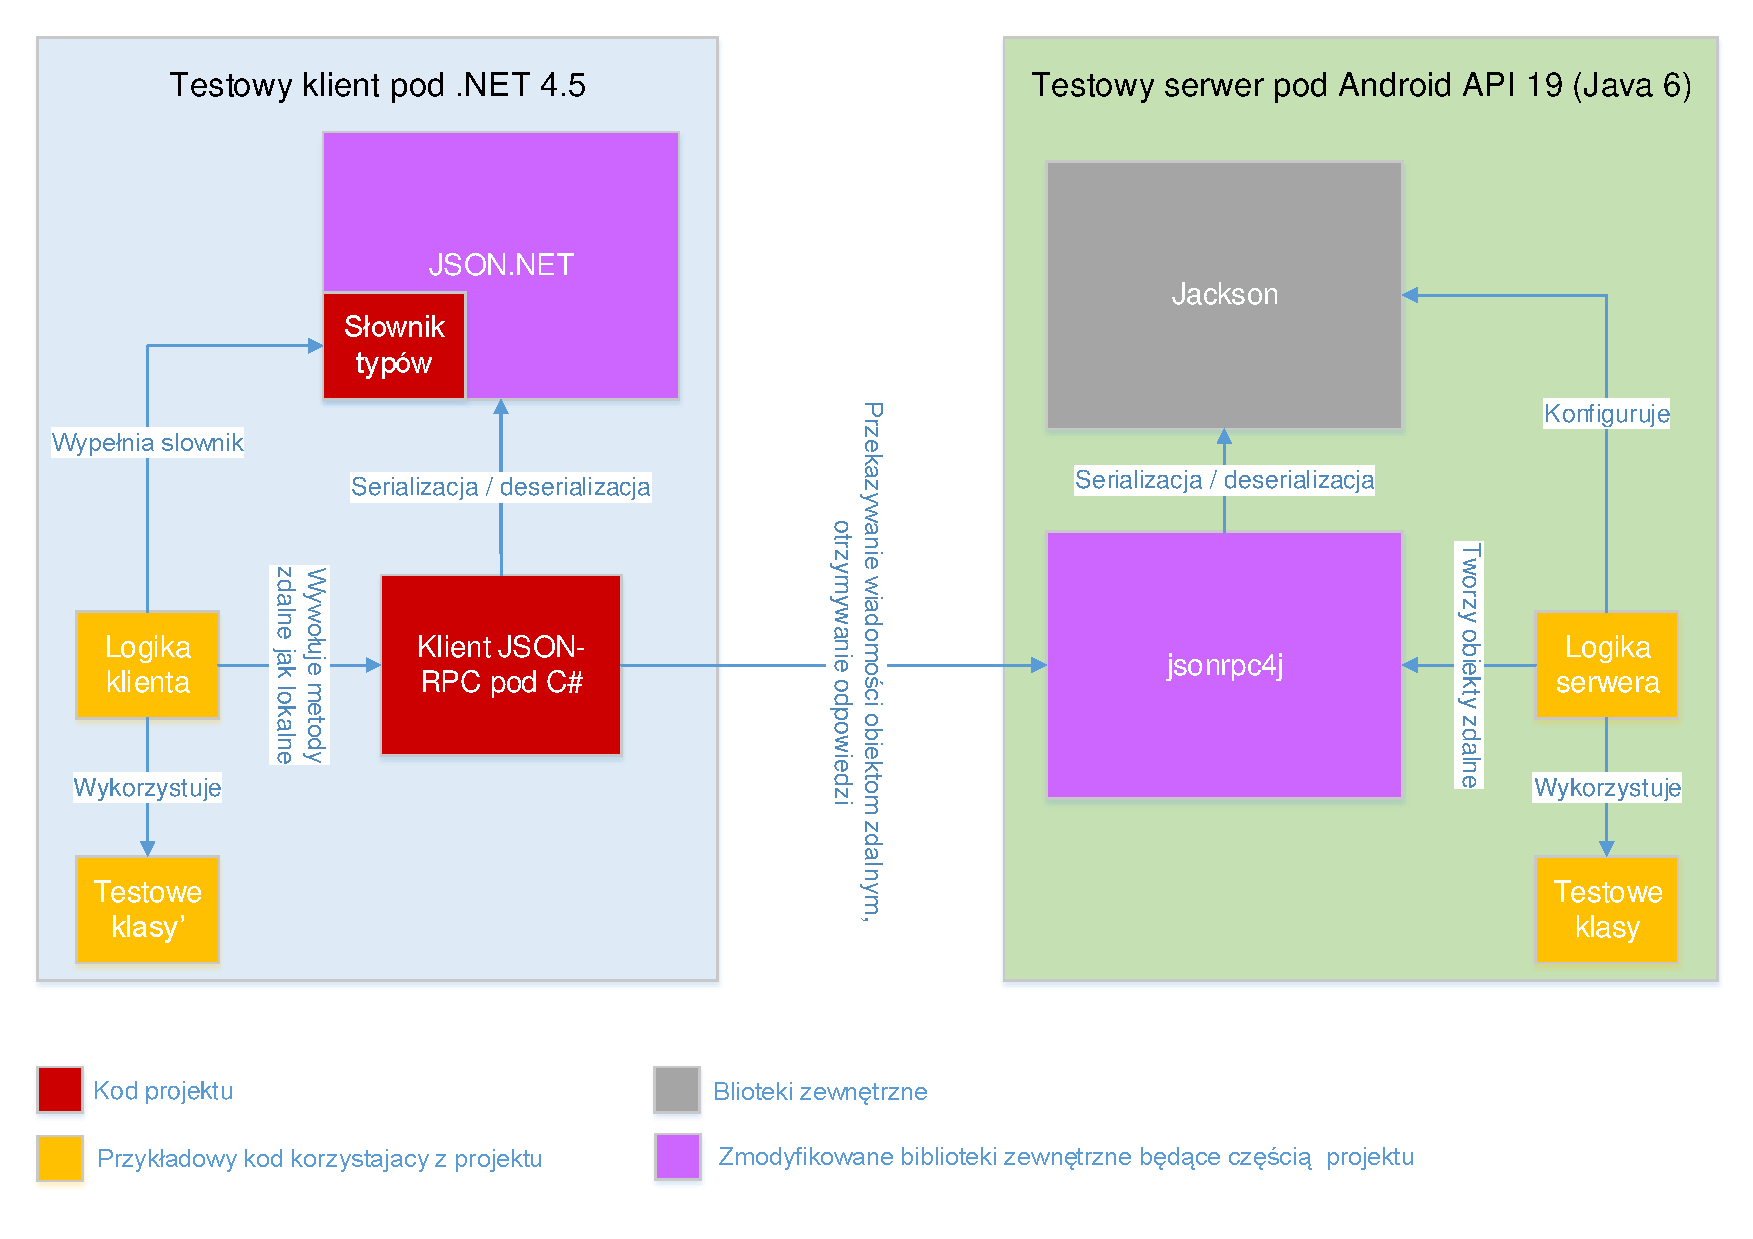
\includegraphics[width=\textwidth]{img/schematy/schemat-implementacji.pdf}
	\caption{Struktura częściowej implementacji projektu.}
	\label{fig:implementation-overview}
\end{figure}

\begin{figure}
	\centering
		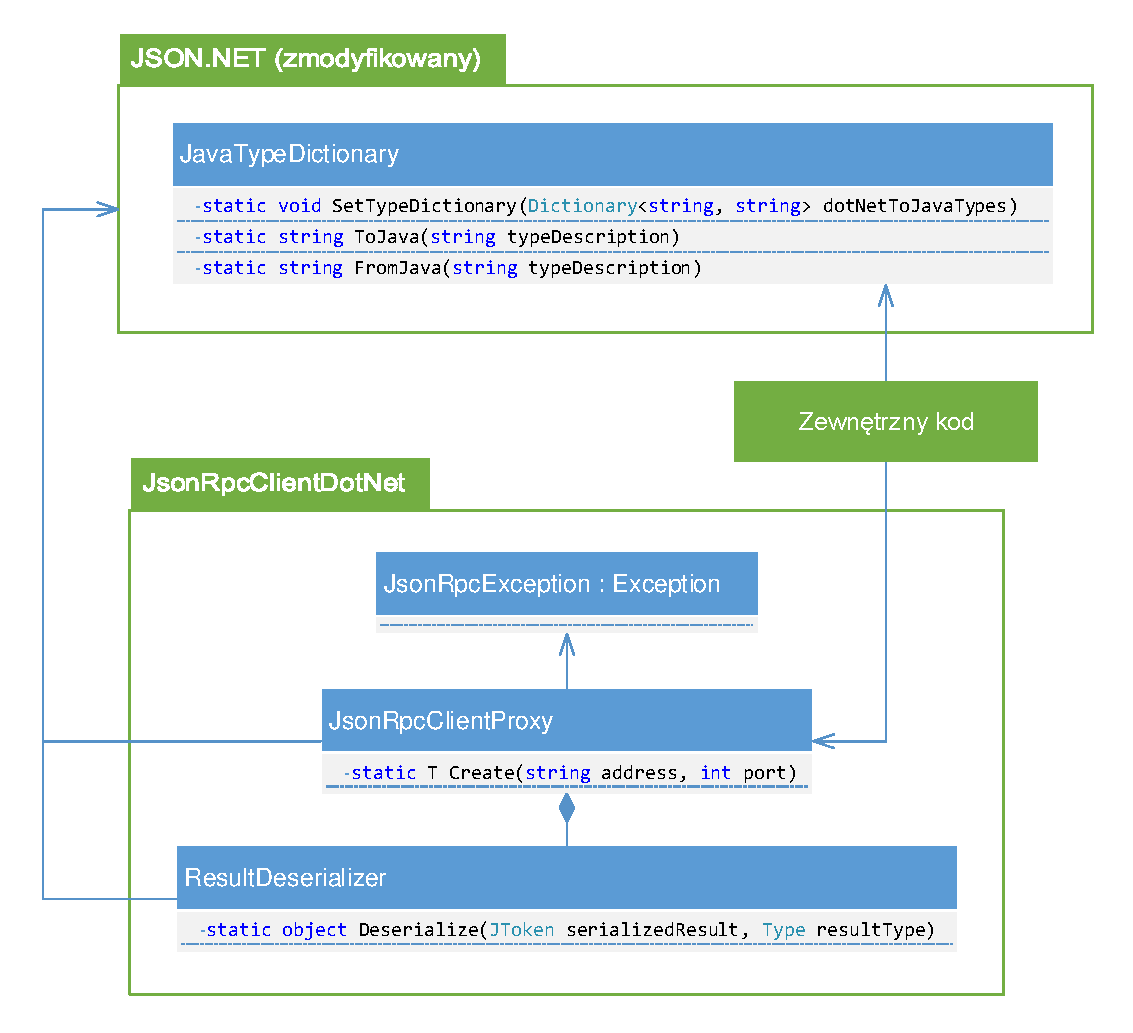
\includegraphics[width=\textwidth]{img/schematy/schemat-klas-net.pdf}
	\caption{Klasy klienta JSON-RPC pod .NET.}
	\label{fig:dot-net-classes}
\end{figure}

\begin{figure}
	\centering
		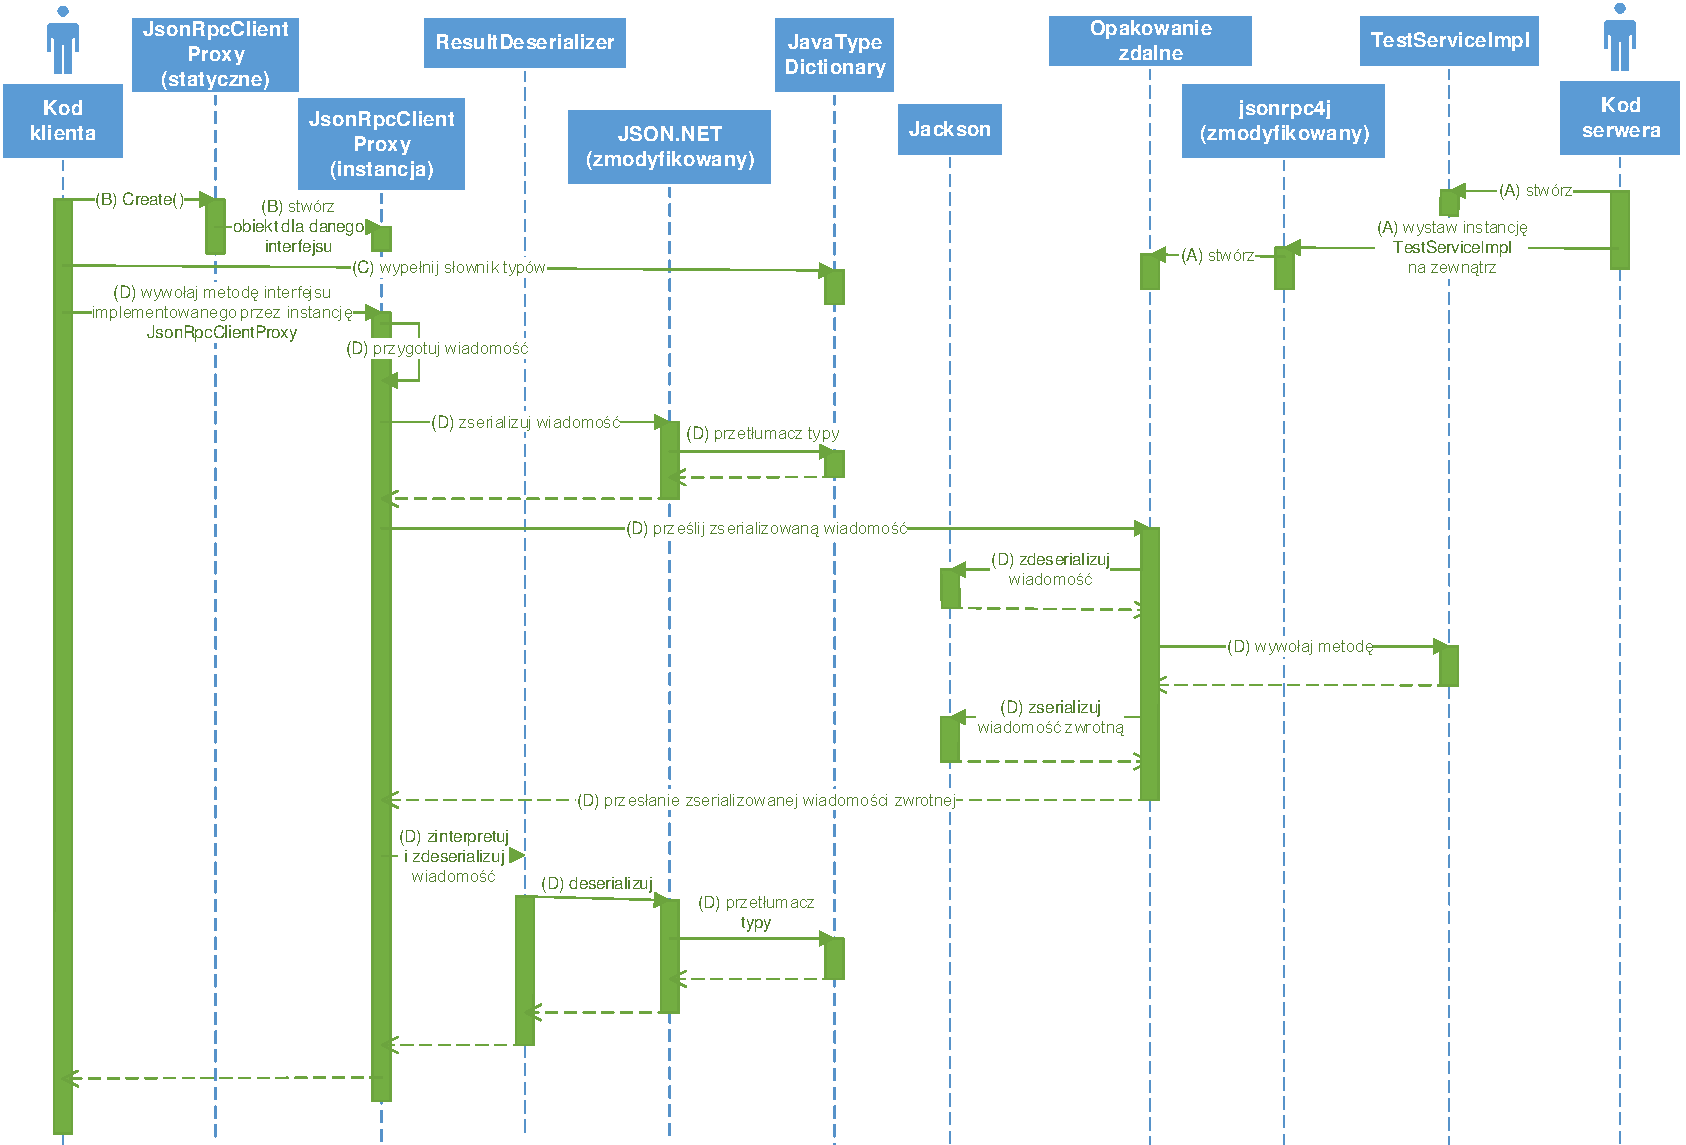
\includegraphics[angle=90,origin=c,scale=0.8]{img/schematy/diagram-sekwencji.pdf}
	\caption[Diagram sekwencji systemu.]{Diagram sekwencji systemu. Są 4 niezależne scenariusze: A, B, C i D. D musi wystąpić po 3 poprzednich.}
	\label{fig:sequence-diagram}
\end{figure}

Sekwencja A to stworzenie obiektu zdalnego. Wyjaśnienie jej kroków:
\begin{itemize}
	\item Kod serwerowy tworzy instancję wybranej klasy, na diagramie jest to \texttt{TestServiceImpl}.
	\item Kod serwerowy wystawia publiczne metody stworzonej instancji \texttt{TestServiceImpl} ,,na zewnątrz'' przy użyciu API jsonrpc4j.
	\item Biblioteka jsonrpc4j tworzy obiekt opakowujący instancję \texttt{TestServiceImpl}; ten obiekt będzie odpowiedzialny za~wołanie metod instancji \texttt{TestServiceImpl} w~odpowiedzi na otrzymywanie wiadomości od klientów JSON-RPC.
\end{itemize}

Sekwencja B -- stworzenie obiektu klienckiego. Faktycznie niezależna od sekwencji A, ponieważ obiekt zdalny musi istnieć dopiero przy pierwszym wywołaniu metody, nie przy stworzeniu obiektu klienckiego. Kroki:
\begin{itemize}
	\item Kod kliencki tworzy instancję obiektu klienckiego (proxy) dla obiektu zdalnego.
	\item Statyczna metoda \texttt{JsonRpcClientProxy} tworzy instancję swojej klasy. Instancja tworzona jest na bazie zadanego interfejsu (np. \texttt{TestService}) i~jest wiązana z~adresem konkretnego obiektu zdalnego.
\end{itemize}

Sekwencja C -- wypełnienie słownika typów. Potrzebne jeśli użytkownik zamierza korzystać z~polimorfizmu parametrów metod zdalnych. Polega na uruchomieniu jednej metody statycznej zmodyfikowanego przeze mnie JSON.NET\footnote{Biblioteka serializacyjna pod .NET; format danych to JSON.}. Wypełniony słownik będzie wykorzystywany do mapowania typów pomiędzy Javą a~.NET przy serializacji i~deserializacji.

Sekwencja D -- wywołanie polimorficznej metody zdalnej, czyli zasadnicza funkcjonalność systemu:
\begin{itemize}
	\item Metoda .NETowej wersji interfejsu \texttt{TestService} wywołana na instancji \texttt{JsonRpcClientProxy} przez kod kliencki. 
	\item \texttt{JsonRpcClientProxy} przygotowuje wiadomość dla serwera JSON-RPC i~zawiera w~niej przekazane argumenty metody zdalnej.
	\item Wiadomość jest przekazana do serializacji do zmodyfikowanego JSON.NET.
	\item Jeśli zachodzi taka potrzeba, JSON.NET pyta \texttt{JavaTypeDictionary} o~nazwy typów w~Javie, które odpowiadają typom parametrów przekazanych do \texttt{JsonRpcClientProxy}.
	\item \texttt{JsonRpcClientProxy} wysyła zserializawoną wiadomość do serwera JSON-RPC opakowującego instancję obiektu zdalnego.
	\item Po odebraniu wiadomości zakodowanej w~JSON, opakowanie obiektu zdalnego przekazuje ją do deserializacji do Jacksona.
	\item Opakowanie obiektu zdalnego przekazuje zdeserializowane parametry do odpowiedniej metody obiektu zdalnego. On wykonuje te metodę lokalnie i~zwraca otrzymaną wartość do obiektu opakowującego.
	\item Obiekt opakowujący przygotowuje zwrotną wiadomość JSON-RPC umieszczając w~niej obiekt zwrócony z~metody zdalnej. Następnie wiadomość jest serializowana przy użyciu Jacksona.
	\item Zserializowana wiadomość jest zwrócona do \texttt{JsonRpcClientProxy}.
	\item \texttt{JsonRpcClientProxy} przekazuje wiadomość do wewnętrznego obiektu \texttt{ResultDeserializer}. \texttt{ResultDeserializer} rozpoznaje, czy zwrócona wartość to wynik metody czy wyjątek.
	\item \texttt{ResultDeserializer} deserializuje zwróconą wartość wyciągniętą z~wiadomości przy użyciu JSON.NET.
	\item JSON.NET prosi \texttt{JavaTypeDictionary} o~przetłumaczenie nazw typów Javy na odpowiadające nazwy w~.NET.
	\item \texttt{JsonRpcClientProxy} przekazuje do kodu klienckiego przetłumaczony obiekt otrzymany z~metody zdalnej.
\end{itemize}



%Co to? Jakie wymagania spełnia? Co by wchodziło w tego skład lub ogólny sposob realizacji? Realizacja prototypu. Ograniczenia?
\section{Polimorfizm a wspólny format informacji o typach}

\subsection{Wprowadzenie}

\subsubsection{Zdalne metody bez polimorfizmu}
Obie części systemu -- klient (.NET) i~serwer (Android) -- muszą mieć wspólny system oznaczania typów, aby wymieniane obiekty mogły być polimorficzne. 
Wspólny format oznaczeń nie jest potrzebny, kiedy nie zależy nam na polimorfizmie, czyli w~większości przypadków wykorzystania zdalnego wywoływania metod (kodu).

Zanim przejdę do przykładów wprowadźmy trochę pseudokodu bazowanego na Javie. Będzie to interfejs obiektu zdalnego, klasa go implementująca oraz klasa danych używana wykorzystywana w~interfejsie; wszystkie znajdujące się w~jednej przestrzeni nazw (\emph{package}). Kod ten znajduje się na listingu~\ref{kod:example-remote-classes}.

\begin{lstlisting}[float, frame=single, caption={Przykładowy kod metody zdalnej.}, label=kod:example-remote-classes]
package org.example.test;

public class DataA
{
    public int number;
    public String text;
}

public interface TestService
{        
    DataA modifyData(DataA data);
}

public class TestServiceImpl
{
    DataA modifyData(DataA data)
    {
        data.number += 1;
        data.text += " something added";
        return data;
    }
}
\end{lstlisting}

Załóżmy, że będziemy wywołać metody za pomocą JSON-RPC. Klasyczne JSON-RPC nie koduje w~żaden sposób informacji o typach. Można by z~.NET przekazać zakodowaną wiadomość, podobną do tej z~listingu~\ref{kod:example-call}, i Java potrafiłaby ją rozkodować. To dlatego, że w~wybranym obiekcie (o~identyfikatorze \texttt{TestServiceImpl1}) istnieje metoda o~nazwie \texttt{modifyData}. Co więcej, przyjmowany przez nią parametr ma dwa obiekty składowe: \texttt{number} i \texttt{text} -- tak samo jak obiekt \texttt{DataA}; dlatego parametr z~JSONa może być zinterpretowany jako \texttt{DataA}\footnote{Zgodnie z~zasadą \emph{Duck Typing}}.

\begin{lstlisting}[frame=single, float, caption={Przykład wiadomości JSON wywołującej metodę zdalną.}, label=kod:example-call]
{
    "obiekt": "TestServiceImpl1",
    "metoda": "modifyData",
    "parametry": [
        {
            "number": 13,
            "text": "przykladowy tekst"
        }
    ]
}
\end{lstlisting}

Gdyby obiekt zdalny był klasyczną, a~więc korzystającą z~SOAP, usługą sieciową (\emph{web service}), to powyższy przypadek nie działałby ,,tak po prostu''.
To dlatego, że we wiadomościach SOAP każdy obiekt danych musi być oznaczonym konkretnym typem XML Schema.
Jest to poważny wysiłek, którego w~powyższym przypadku ani serwer, ani klient nie muszą podejmować.

\subsubsection{Zapotrzebowanie na polimorfizm}
\label{need-for-polymorphism}
Póki co, kodowanie informacji o~typach nie jest do niczego potrzebne. Wprowadźmy teraz nową klasę, która dziedziczy po \texttt{DataA} (listing~\ref{kod:example-inheritance}).
Zakładamy też, że po stronie .NET znajduje się odpowiednik zarówno \texttt{DataA}, jak i~dziedziczącej po nim \texttt{DataB}. Także relacja dziedziczenia jest zachowana pomiędzy odpowiednikami. Nazwijmy te odpowiedniki \texttt{DataA'} i~\texttt{DataB'}.

\begin{lstlisting}[frame=single, float, caption={Klasa danych dziedzicząca po innej klasie danych.}, label=kod:example-inheritance]
package org.example.test;

public class DataB extends DataA
{
    public double floatNumber;
}
\end{lstlisting}

Powiedzmy, że teraz klient chce wywołać metodę \texttt{modifyData} przekazując jako parametr \texttt{DataB'}, a~nie \texttt{DataA'} (które było interpretowane przez serwer jako \texttt{DataA}), jak poprzednim razem.
W~programowaniu obiektowym nie jest to nic dziwnego -- polimorfizm powinien zapewniać to, że obiekt dziedziczący może być zinterpretowany jako bazowy.
Wynikająca z~takiego wywołania wiadomość znajduje się na listingu~\ref{kod:bad-inheritance-call}.

\begin{lstlisting}[frame=single, float, caption={Wywołanie zawierające parametr dziedziczący po parametrze spodziewanym.}, label=kod:bad-inheritance-call]
{
    "obiekt": "TestServiceImpl1",
    "metoda": "modifyData",
    "parametry": [
        {
            "number": 13,
            "text": "przykladowy tekst",
            "floatNumber": 5.25
        }
    ]
}
\end{lstlisting}

Wiadomość ta różni się od poprzedniej tylko polem \texttt{floatNumber}. W~tej sytuacji serwer może się zachować dwojako, w~zależności od konfiguracji.
Może stwierdzić, że nie ma metody \texttt{modifyData} przyjmującej jeden parametr, który posiada trzy pola: \texttt{number}, \texttt{text} i~\texttt{floatNumber}. W~tej sytuacji nie zostanie wywołana żadna metoda zdalna, a~serwer powinien zwrócić klientowi wyjątek.
Drugim wyjściem jest pominięcie nierozpoznanego przez serwer \texttt{floatNumber} i~zinterpretowanie reszty pól jako obiektu \texttt{DataA}.
Metoda wykona się poprawnie, ale może być to działanie niepożądane przez programistę. Przekazując metodzie instancję \texttt{DataB'} mógł chcieć, żeby obiekt zdalny użył faktycznie jej\footnote{Nie jest, oczywiście, możliwe użycie tej samej instancji obiektu, którą przekazał klient. Chodzi o~dokładną kopię.}. Gdyby działanie metody zależało od typu jej parametru, np. kiedy dokonywana jest inspekcja parametru przy użyciu refleksji, to metoda nie zadziałałaby tak, jak oczekiwał tego programista.

Oczywista jest przydatność polimorfizmu gdyby na przyjmowanym parametrze była wywoływana jakaś metoda. Jest to standardowy sposób rozszerzania działania kodu bez jego przepisywania, stosowany w~programowaniu obiektowym.
Klasy, które tutaj nazywam ,,klasami danych'' i~używam jako argumentów dla metod zdalnych mogą mieć metody, jednak wprowadza to problem przy utrzymywaniu bliźniaczych klas we dwóch językach.

Łatwo jest przepisać na inny język klasę, które posiada tylko pola i~żadnych metod -- może to często zrobić nawet automat.
Metody, natomiast, mogą być wyzwaniem nawet dla człowieka. Nawet, jeśli mowa o~prostej logice, to utrzymanie równoznaczności metod w~obu językach może być wymagające.
Co prawda, równoznaczność nie jest wcale niezbędna. Po obu stronach systemu klasa może mieć zupełnie inne metody i~zachowanie, zachowując te same pola. Ma to jednak wyraźnie zły wpływ na przejrzystość kodu całego systemu.

Aby obronić polimorfizm w~obiektach zdalnych, mogę dać nieco wydumany przykład metody, która rysuje koła, a~jest sparametryzowana obiektem typu \texttt{Object} (czyli dowolnym). Domyślnie rysuje ona jedno koło o promieniu 5.0, ale w~przekazanym obiekcie szuka pól \texttt{int} (żeby pierwszy \texttt{int} został zamieniony na ilość kół) i \texttt{double} (żeby pierwszy \texttt{double} został zamieniony na promień rysowanych kół).
Inspekcja obiektów może być używana chociażby przy różnego rodzaju konfiguracjach. Np.\ każdy obiekt hipotetycznego typu \texttt{AdresBazyDanych} znajdujący się w~przychodzących do metod zdalnych parametrach ma zostać podmieniony na wartość pożądaną przez serwer. Kiedy dalej obiekt zdalny będzie wykonywać jakieś operacje na przesłanych parametrach, to będzie używany adres skonfigurowany na serwerze, a~nie jakiś nieznany przysłany z~zewnątrz.
Mniej więcej tak dzieje się w~Spring IoC~\cite{sping-ioc} -- kontenerze odpowiedzialnym za automatyczną konfigurację aplikacji webowej opartej na frameworku Spring.

%Aby programista nie tracił niespodziewanie żadnych danych i miał po drugiej stronie to, czego chce
%Aby sytuacja była jasna typy muszą być oznaczane. Do tego, oznaczanie typów musi być jednolite. Musi być słownik itp. Wtedy wiadomość wyglądałaby tak, bo klient by sobie przetłumaczył typy (zakładamy, że robi to klient). Serwer by sobie odebrał i byłoby git.
%


\subsection{Plan rozwiązania}
W~ogólności -- aby polimorfizm metod zdalnych był możliwy potrzeba, aby klient i~serwer:
\begin{itemize}
	\item oznaczały typy obiektów, kiedy nie są one jednoznaczne;
	\item oznaczały typy w~sposób zrozumiały dla drugiej strony;
	\item miały dostęp do typów odpowiadającym typom przesyłanym z~drugiej strony (typy lustrzane).
\end{itemize}

O~lustrzanych typach pisałem już we wprowadzeniu powyżej. Przykładowy program w~Javie posiadał typy \texttt{DataA} i~\texttt{DataB} po nim dziedziczący. Kod pod .NET posiadał, natomiast, odpowiadające im \texttt{DataA'} i~\texttt{DataB'}.
Przy założeniu, że używanym przez nas językiem platformy .NET będzie C\#, powstanie klasa z~listingu~\ref{kod:dot-net-data-classes}.

\begin{lstlisting}[frame=single, float, caption={Przykładowe klasy danych zapisane w~C\#}, label=kod:dot-net-data-classes]
namespace SerializationTest
{
  public class DataA
  {
      public int number;
      public string text;
  }
  
  public class DataB : DataA
  {
      public double floatNumber;
  }
}
\end{lstlisting}

W tym przypadku Java (listingi~\ref{kod:example-remote-classes} i~\ref{kod:example-inheritance}) i~C\# (listing~\ref{kod:dot-net-data-classes}) są do siebie bardzo zbliżone.

Można zauważyć kilka rzeczy:
\begin{itemize}
	\item Nazwy klas nie zawierają prim (') -- będą używane tylko w~skróconych oznaczeniach w~tekście.
	\item Nazwa paczki Javy (\texttt{org.example.test}) i~przestrzeń nazw z~.NET (\texttt{SerializationTest}) nie są takie same; pełne nazwy klas będą następujące: dla Javy -- \texttt{org.example.test.DataA} i~\texttt{org.example.test.DataB}, dla .NET -- \texttt{SerializationTest.DataA} i~\texttt{SerializationTest.DataB}.
	\item Klasy z~C\# zachowują zależność dziedziczenia.
	\item Odpowiadające sobie klasy mają taki sam zestaw publicznych pól; ważny jest ich typ i nazwy, nie jest ważna kolejność.
	\item Mimo tego, że tutaj odpowiadające sobie klasy mają takie same nazwy, to nie jest to potrzebne (choć zapewnia czytelność).
	\item Aby logicznie powiązać odpowiadające sobie klasy musi istnieć pewnego rodzaju słownik; to on pokaże, że np. \texttt{org.example.test.DataA} jest odpowiednikiem \texttt{SerializationTest.DataA}; zależność ta jest wzajemna.
\end{itemize}

%Oznaczanie typów wymaga słownika. Można by wymusić takie same namespace'y i package, ale każde mają inne zasady nazewnictwa. Można by też wprowadzić identyfikacje po ostatnim członie, ale wtedy stracilibyśmy korzyść z osobnych przestrzeni nazw.

Odpowiadające sobie typy danych w~językach tak podobnych jak Java i~C\# mogłyby teoretycznie być uzyskiwane przez automatyczne tłumaczenie -- z~Javy do .NET lub odwrotnie.
Nie udało mi się jednak uruchomić żadnego narzędzia, które powinno to potrafić.

Oznaczenie typów może polegać na dodawaniu do obiektu specjalnego pola. W~przykładzie z~listingu~\ref{kod:call-with-types}, przedstawiającym hipotetyczną wiadomość wysłaną z~.NET, to pole zostało nazwane \texttt{\$typ} i~posiada wartość typu \emph{string} zawierającą pełną, jednoznaczną nazwę typu.

\begin{lstlisting}[frame=single, float, caption={Przykład wywołania zdalnej metody zawierającego informację o~typach.}, label=kod:call-with-types]
{
    "obiekt": "TestServiceImpl1",
    "metoda": "modifyData",
    "parametry": [
        {
            "$typ": "SerializationTest.DataB"
            "number": 13,
            "text": "przykladowy tekst",
            "floatNumber": 5.25
        }
    ]
}
\end{lstlisting}

Po dodaniu takiego pola serwer powinien wiedzieć jaki konkretnie obiekt otrzymał.
Gdyby przekazano obiekt \texttt{DataA} to informacja o~typie (pole \$typ) nie byłaby potrzebna, ponieważ \texttt{DataA} jest spodziewanym typem parametru metody \texttt{modifyData}.


\subsection{Implementacja}
\subsubsection{Założenia}
Od razu zakładam, że serializacja danych będzie oparta o~JSON a~protokołem komunikacyjnym będzie JSON-RPC. Pozwoli to na lekką komunikację i~stosunkowo prostą implementację.
Ponadto, biblioteka JSON-RPC dla języka Java -- jsonrpc4j\footnote{Patrz punkt~\ref{jsonrpc4j}.}, może po modyfikacji działać na Androidzie.
Po stronie .NET posłużę się otwartą biblioteką do serializacji do JSON -- JSON.NET.

Jackson jest biblioteką serializacyjną z~której korzysta jsonrpc4j. Zarówno Jackson jak i~JSON.NET mają dużo możliwości konfiguracji. Obie posiadają też możliwość kodowania (przez specjalne pola) informacji o~typach (listing~\ref{kod:serilization-objects}).

\subsubsection{Porównanie działania Jackson i~JSON.NET}
Zestawienie ich działania dla kilku przypadków znajduje się na listingach~\ref{kod:serilization-objects}, \ref{kod:serialization-arrays}, \ref{kod:serialization-lists}, \ref{kod:serialization-dicts}. Różnice stylu oznaczania typów są w~tabeli~\ref{tab:jackson-jsonnet-differences}

\begin{lstlisting}[float, frame=single, caption={Porównanie serializacji obiektów typu \texttt{DataA}}, label=kod:serilization-objects]
\\ Jackson
{
    "@class":"org.example.test.DataA",
    "number":13,
    "text": "przykladowy tekst"
}

\\ JSON.NET
{
    "$type": "SerializationTest.DataA, TestDataLib",
    "number": 13,
    "text": "przykladowy tekst"
}
\end{lstlisting}

\begin{lstlisting}[float, frame=single, caption={Porównanie serializacji tablicy obiektów typu \texttt{Object}. Tablica zawiera wartość typu \texttt{int} oraz wartość typu \texttt{string}}., label=kod:serialization-arrays]
\\ Jackson
[
  "[Ljava.lang.Object;",
  [
    28,
    "jakis tekst"
  ]
]

\\ JSON.NET
{
  "$type": "System.Object[], mscorlib",
  "$values": [
    28,
    "jakis tekst"
  ]
}
\end{lstlisting}

\begin{lstlisting}[float, frame=single, caption={Porównanie serializacji listy obiektów typu \texttt{Object}. Lista zawiera wartość typu \texttt{int} oraz wartość typu \texttt{string}}., label=kod:serialization-lists]
\\ Jackson
[
  "java.util.ArrayList",
  [
    28,
    "jakis tekst"
  ]
]

\\ JSON.NET
{
  "$type": "System.Collections.Generic.List`1
	                     [[System.Object, mscorlib]], mscorlib",
  "$values": [
    28,
    "jakis tekst"
  ]
}
\end{lstlisting}

\begin{lstlisting}[float, frame=single, caption={Porównanie serializacji słownika/mapy (\emph{dictionary/map}) mapującego wartość typu \texttt{string} do wartości typu \texttt{int} (\texttt{int} jest kluczem).}, label=kod:serialization-dicts]
\\ Jackson
{
  "@class":"java.util.HashMap",
  "1":"pierwszy",
  "2":"drugi",
  "3":"trzeci"
}

\\ JSON.NET
{
  "$type": "System.Collections.Generic.Dictionary`2
	          [[System.Int32, mscorlib],[System.String, mscorlib]],
            mscorlib",
  "1": "pierwszy",
  "2": "drugi",
  "3": "trzeci"
}
\end{lstlisting}

\begin{table}[htbp]              
	\centering
	\caption{Różnice w~stylu oznaczania typów pomiędzy Jackson a JSON.NET.}
		\begin{tabular}{ | p{0.25\textwidth} || p{0.25\textwidth} | p{0.40\textwidth} | }
			\hline
				& \textbf{Jackson} & \textbf{JSON.NET} \\
				\hline \hline
				Nazwa pola specjalnego pola zawierającego oznaczenie typu & \texttt{@class} & \texttt{\$type}. \\
				\hline
				Oznaczenie typu zawiera & Pełną nazwę klasy & Pełną nazwę klasy oraz nazwę źródłowej biblioteki (DLL). \\
				\hline
				Oznaczenie typu list i~tablic & Opakowanie w~dodatkową listę, której pierwszym elementem jest \texttt{string} z~nazwą typu, a~drugim oryginalna kolekcja. & Opakowanie w~obiekt z~dwoma polami: \texttt{\$type} i~\texttt{\$values} zawierającym oryginalną kolekcję. \\
				\hline
				Oznaczenie typów generycznych & Nie ma i~nie jest możliwe ze względu na \emph{,,type erasure''}. & Oznaczane przy użyciu składni <nazwa-typu-generycznego>`<ilość-parametrów-typu>[[<nazwa-typu-1>], [<nazwa-typu-2>], ...] \\
				\hline
		\end{tabular}
	\label{tab:jackson-jsonnet-differences}
\end{table}

\subsubsection{Dookreślenie planu rozwiązania}
Mimo, że JSON.NET posiada duże możliwości konfiguracji stylu serializacji, zdecydowałem się na modyfikację jego źródeł, zamiast pisania biblioteki na nim bazującej. Nie wszystko da się zrobić przez konfigurację, np.\ nie da się zmienić nazwy specjalnego pola z~typem (\texttt{\$type}).
Wydaje się też, że zbudowanie programu imitującego sposób serializacji Jacksona korzystającego z~JSON.NET byłoby znacznie bardziej pracochłonne niż przerobienie JSON.NET, aby robił to samo.

Zmodyfikowany JSON.NET traci zgodność ze swoim niezmodyfikowanym odpowiednikiem.
Przestają też działać niektóre zaawansowane funkcje, np. zapisywanie referencji do obiektów znajdujących się w~pamięci.
Można je pominąć, ponieważ nie są przydatne w~moim zastosowaniu, tj.\ w~serializacji obiektów danych, które mają być wysyłane na inną platformę.

Aby JSON.NET miał wspólny z~Jackson format informacji o~typach trzeba:
\begin{itemize}
	\item zmienić nazwę pola oznaczającego typ z~\texttt{\$type} na @class;
	\item zmienić sposób serializacji tablic i~list na taki, który imituje Jacksona;
	\item zmienić sposób deserializacji tablic i~list, aby mogły być przyjmowane od Jacksona;
	\item utrzymywać po obu stronach (Java, C\#) odpowiadające sobie klasy danych;
	\item stworzyć słownik łączący pełne nazwy klas w~Javie z~odpowiednikami w~.NET i~vice versa.
\end{itemize}

Brak informacji o~konkretnym typie typów generycznych zserializowanych Jacksonem będzie problemem, jeśli po drugiej stronie typ ten nie będzie mógł być jednoznacznie wywnioskowany. Np.\ kiedy nie ma żadnych założeń co do typu obiektu -- będzie to typ dziedziczący po \texttt{Object}.
Powiedzmy, że zserializowano obiekt, którego jedno pole ma typ generyczny, np.\ jako pole typu \texttt{ArrayList<String>}. W~takim przypadku konkretny typ szablonu \texttt{ArrayList} będzie mógł być wywnioskowany i~system będzie działał dobrze.
Ogólnie -- wrodzoną wadą systemu będzie to, że typy generyczne nie zawsze będą działać.
Nie jest to winą Jacksona, a~mechanizmu języka Java zwanego \emph{,,type erasure''} usuwającego informacje o~faktycznym typie typu generycznego w~trakcie wykonywania kodu.

Jackson nie obsługuje też informacji o bibliotece. Schemat nazywania pakietów w~Javie powinien jednak zapewniać ich unikatowość, więc brak nazwy biblioteki to nie problem.

\subsubsection{Ostateczny kształt rozwiązania}
JSON.NET ma 14401 linii kodu, używany przeze mnie podzbiór Jackson -- 63497. Obie biblioteki są dobrze napisane i~konfigurowalne, ale nie zakładają dużej ingerencji w~system oznaczania typów, który to w~obu przypadkach jest inny i~specyficzny.

W~przypadku JSON.NET, który próbowałem zmodyfikować mechanizmy wykrywania i~oznaczania typów są dość mocno uwiązane z~resztą biblioteki.
Z~racji natury procesów serializacji i~deserializacji kod jest rekurencyjny i~mocno rozgałęziony.
To sprawia, że ciężko wykonać większą modyfikację bez skutków ubocznych w~kodzie.
Przez to nie udało się dopasować serializacji tablic i~list do formatu Jacksona. Zdecydowanie nie jest to niemożliwe, ale wysiłek do tego potrzebny nie zmieścił się w~ramach tej pracy.

Całkowicie, natomiast udała się serializacja dowolnych pojedynczych (nawet skomplikowanych) obiektów. Dzięki temu można uzyskać sprawne polimorficzne metody zdalne.

Wykonane modyfikacje JSON.NET według klas:
\begin{description}
\itemtitle{\texttt{JavaTypeDictionary}}
Stworzona przeze mnie w~całości klasa statyczna. Można ją zainicjować za pomocą słownika, czyli obiektu typu \texttt{Dictionary}. Klasa go zapamiętuje oraz tworzy słownik odwrotny (klucze i~wartości zamienione rolami) dla szybszego przeszukiwania. Klasa ta będzie używana przez resztę JSON.NET do tłumaczenia nazw typów.

\itemtitle{\texttt{JsonSerializerInternalWriter}}
W~metodzie \texttt{WriteTypeProperty} dodano tłumaczenie zapisywanych nazw typów na odpowiedniki z~Javy.

\itemtitle{\texttt{JsonTypeReflector}}
Stała \texttt{TypePropertyName} zmieniona z~\texttt{\$type} na \texttt{@class}, aby zapewnić zgodność z~Jacksonem. JSON.NET rozpoznaje specjalne pola obiektów po tym, że zaczynają się od ,,\$''. Dlatego ta zmiana psuje zgodność z~oryginalnym JSON.NET.

\itemtitle{\texttt{JsonSerializerInternalReader}}
Metoda \texttt{ReadMetadataProperties} stosowała wspomniany wcześniej mechanizm wykrywania specjalnych pól obiektów polegający na sprawdzaniu, czy  pierwszy znak nazwy to ,,\$''. Został on zamieniony na ,,@'', aby mogło być wyłapane pole \texttt{@class}. Ponadto, metoda \texttt{ResolveTypeName} korzysta z~\texttt{JavaTypeDictionary} do tłumaczenia nazw klas z~Javy na .NET.
\end{description}
Łącznie, zmodyfikowałem 7 linii i~dodałem 44, aby uzyskać oznaczanie typów zgodne z~Jacksonem dla pojedynczych obiektów.
Modyfikacja serializacji i deserializacji kolekcji byłaby dużo bardziej złożona.

%Żeby słownik był dobry dla programisty, to dobrze jakby
%Potrzebny jest system mapujący nazwy typów w jednym środowisku, na nazwy z drugiego. Mógłby działać na zasadzie słowników. Żeby zmniejszyć nakład pracy mogły by one być generowane automatycznie zgodnie z jakąś zasadą.
%Pewnie potrzebny by był też system ładowania klas.
%Może jakiś schemacik tego ładowania i jakby mapowanie działało przy serializacji, deserializacji.

%Potrzebny byłby system ładowania bibliotek i klas z nich. Ale i tak nie dostarczam gotowego systemu, tylko taki prototyp, wiec chyba mogę to pominąć. Tłumaczenia klas też nie będzie. Albo tłumaczenie mogę pominąć, ładowanie zrobić konfigurowane, tj. tak jak słownik typów byłby spis bibliotek (np. z ich pełnymi ścieżkami). Te biblioteki byłyby ładowane do Assembly w .NET i do aktualnego class loadera w javie. Można by to prosto obtestować.



\section{Zdalne wywoływanie metod na Androidzie}
\label{android-rpc}

\subsection{Wybrana forma zdalnego wywoływania metod}
Jako format zdalnego wywoływania metod w~moim systemie wybrałem JSON-RPC 2.0. Przez swoją prostotę zyskuje on odporność na błędy i~łatwość implementacji.
Poza tym spełnia wszystkie założone wymagania -- identyfikuje docelowe obiekty i~metody oraz pozwala rozszerzać sposób serializacji parametrów metod.
Każda wiadomość posiada też identyfikator, który wspomaga rozumienie serii wiadomości w~wymianie między klientem a serwerem jako logicznej ,,rozmowy''.

Ponadto od wersji 2.0, JSON-RPC posiada mechanizm rozszerzania swoich wiadomości (\emph{Extensions})~\cite{json-rpc-extensions}.
Dzięki tym rozszerzeniom można by wyróżnić pewne szczególne wiadomości dla serwera, np.\ takie, które mają wywołać stworzenie nowej instancji zdalnego obiektu lub usunięcie starej.
Taka funkcjonalność jest zawarta w~zebranych wcześniej wymaganiach systemowych, jednak jako mało kluczowa została poświęcona na rzecz realizacji działającego prototypu.

Jednakże kluczowym elementem, który przyczynił się do decyzji o~użyciu JSON-RPC było istnienie biblioteki jsonrpc4j (opisanej w~punkcie~\ref{jsonrpc4j}). Była prosta w~użyciu, funkcjonalna i~nie brakowało jej dużo, aby mogła działać na Androidzie.


\subsection{Plan rozwiązania}
Gdyby nie skupiać się na polimorfizmie, to, poza zwykłym JSON-RPC, część serwerowa mojego prototypu nie potrzebuje niczego więcej.
Wystarczy stworzyć obiekt posiadający publiczne metody i~wystawić go na zewnątrz za pomocą klasy \texttt{JsonRpcServer} z~jsonrpc4j.
W~tym momencie dowolny klient JSON-RPC, napisany w~dowolnym języku, może wywoływać kod na serwerze.
Jeśli tym serwerem jest Android, a~tak będzie w~tym przypadku, to klient JSON-RPC może zdalnie wykorzystywać API Androida i~nim zarządzać. A~więc spełnione jest jedno z~wymagań.

Trzeba tylko pamiętać o~posiadaniu po obu stronach wyglądających tak samo typów (wyjaśnione w~punkcie~\ref{need-for-polymorphism}).
Chyba, że wszystkie przyjmowane i~zwracane przez zdalne metody typy są typami prostymi (\texttt{int}, \texttt{double}, \texttt{bool}, też \texttt{string}) -- są one powszechnie dostępne i~rozumiane, więc nie będzie żadnych problemów.

Klasa \texttt{JsonRpcServer} umożliwia przyjmowanie połączeń do obiektu zdalnego na kilka sposobów, jednak wszystkie poza jednym wymagają bibliotek, które nie są dostępne dla Androida, tylko dla standardowej (właściwie nawet rozszerzonej o~Javę EE) Javy.
Sposób, który może działać na Androidzie polega na powiązaniu obiektu z~socketem TCP. Obiekt dostaje jeden port, na którym nasłuchuje wiadomości.
Klienci wysyłają zakodowane JSONem wiadomości, po nawiązaniu połączenia TCP z~konkretnym portem, na konkretnym adresie IP.
Na jednym serwerze może być wystawionych tyle obiektów zdalnych, ile jest portów TCP na wszystkich interfejsach sieciowych hosta.
W~przypadku Androida zazwyczaj jest tylko jeden interfejs, co i~tak daje dziesiątki tysięcy portów.

Trzeba ustawić zgodne polimorficzne serializatory zarówno dla klienta jak i~serwera i~wywołać jakąś z~metod, którymi testowałem polimorfizm w~rozdziale~\ref{similar-technologies}.

Kiedy zaczyna nam zależeć na polimorfizmie metod zdalnych, trzeba zwrócić uwagę na konfigurację serializatorów.
Jackson, który jest biblioteką serializacyjną używaną przez jsonrpc4j ma zdolność oznaczania typów. API jsonrpc4j pozwala, na szczęście, na konfigurację parametrów Jacksona. Czyli możemy sprawić, że serwer będzie zarówno rozumiał oznaczenia typów, jak i~sam będzie je stosował.

Polimorfizm ma swoją cenę -- serwer przestaje być uniwersalnie zgodny z~klientami, ponieważ informacje o~typie w~wiadomościach JSON nie są częścią standardu JSON-RPC 2.0.
Aby móc rozmawiać z~serwerem, klient musi teraz mieć tak samo działający serializator.
Jest to proste dla innych aplikacji korzystających z~Jacksona, chociaż ich twórcy musieliby je świadomie skonfigurować. Ale inne biblioteki albo w~ogóle nie potrafią oznaczać typów, albo robią to w~niezgodny sposób.
Tak było w~przypadku JSON.NET, który jednak udało mi się (częściowo) dopasować do Jacksona. 


\subsection{Realizacja}
Przy próbie uruchomienia jsonrpc4j na Androidzie od razu wystąpił błąd. Okazało się, że mimo tego, co jest napisane na stronie projektu\footnote{,,(\ldots)In fact, the client and server both work in an Android environment.(\ldots)~\cite{jsonrpc4j}} nie można uruchomić serwera na Androidzie.
To dlatego, że klasa \texttt{JsonRpcServer} zawiera zależności do bibliotek, które nie są dostępne dla Androida, a~Java musi móc je załadować, kiedy ładuje klasę.

Na szczęście można było podzielić klasę na dwie części -- tę podstawową, która umożliwia wystawianie obiektów zdalnych na portach TCP i~tę zaawansowaną, która dziedziczy po podstawowej i~zależy od bibliotek niedostępnych Androidowi.
Wydzieloną klasę bazową nazwałem \texttt{JsonRpcBasicServer}. Aby wystawić zdalny obiekt wystarczy kod przedstawiony na listingu~\ref{kod:android-remote-object}.

\begin{lstlisting}[float, frame=single, caption={Tworzenie obiektu zdalnego za pomocą jsonrpc4j dostosowanego do Androida.}, label=kod:android-remote-object]
TestServiceImpl service = new TestServiceImpl();
JsonRpcBasicServer serverBase = new JsonRpcBasicServer(
    ServerThread.createMapper(),
    service,
    TestService.class);
		
bindAddress = InetAddress.getByName("0.0.0.0");
StreamServer server = new StreamServer(
    serverBase,
    maxThreads,
    port,
    0,
    bindAddress);

server.start();
\end{lstlisting}

Tym samym serwer jest całkowicie sprawny i~umożliwia wystawianie dowolnych metod Javy (poza metodami generycznymi) do wykorzystania dla wszystkich klientów JSON-RPC.
Ponieważ po moich zmianach nie ma żadnego spadku funkcjonalności będę próbował przyłączyć je do oryginalnego projektu.



\section{Klient JSON-RPC pod .NET}
\subsection{Podstawy}
Kod kliencki mojego systemu potrzebuje możliwości wołania serwera JSON-RPC.
Okazuje się, że implementacje w~.NET, np. JSON-RPC.NET nie posiadają takiej możliwości.
Potrafią łatwo wystawiać obiekty zdalne na zewnątrz, ale nie mają właściwie żadnych udogodnień do ich konsumowania.
Istnieją jedynie dyskusje na temat części klienckiej i~dość prymitywne ich implementacje.
Te implementacje i~tak zmuszają do ,,własnoręcznego'' złożenia wiadomości JSONowej~\cite{json-rpc-net-client}.

W~przypadku rozwiniętych \emph{frameworków} jak WCF, czy JAX-WS normalne jest, że można w~prosty sposób stworzyć obiekt proxy do serwisu zasilając go jakimś interfejsem.
Następnie obiekt ten może być wołany jak zwykły obiekt lokalny spełniający zadany interfejs.
Taką funkcjonalność posiada też jsonrpc4j.

Postanowiłem stworzyć kod, który pozwoli na eleganckie tworzenie obiektów klienckich i~zdalne wywoływanie metod na tych obiektach.

\subsection{Realizacja}
Udało mi się stworzyć klienta, który jest bardzo wygodny w~użyciu (listing~\ref{kod:my-json-rpc-clinet}).
Można go tworzyć i~wykorzystywać jak normalny obiekt. Zwraca też normalne obiekty.
Jeśli połączy się go ze zmodyfikowanym przeze mnie JSON.NET, to potrafi także przekazywać polimorficzne parametry do mojego serwera.


Implementacja ma ok. 140 linii kodu.
Niestety nie ma jeszcze zaawansowanej logiki odpowiadającej za odporność połączenia, czy ponowne próby wysłania wiadomości. Jeśli coś pójdzie nie tak w~warstwie TCP to zostanie rzucony wyjątek i~wywołanie metody się nie uda.
Nie jest to jednak duża wada.

Podobnie tłumaczenie typów wyjątków nie jest jeszcze wspierane.
To dlatego, że nie są one przekazywane tak, jak normalne obiekty i~wymagają specjalnego sposobu dekodowania (patrz listing~\ref{kod:json-rpc-exception}).
Jeśli coś pójdzie nie tak w~wykonywaniu zdalnej metody (też nie zostanie ona znaleziona), mój klient rzuca ogólny wyjątek \texttt{JsonRpcException}, który zawiera w~sobie wiadomość i~typ wyjątku rzuconego po drugiej stronie.
Idealnie byłoby, gdyby na bazie wiadomości z~błędem otrzymywanej od serwera klient tworzył odpowiednią instancję wyjątku i~go propagował.

\begin{lstlisting}[float, frame=single, caption={Tworzenie obiektu proxy do obiektu zdalnego przy użyciu mojej implementacji klienta JSON-RPC pod .NET.}, label=kod:my-json-rpc-clinet]
TestService service = JsonRpcClientProxy<TestService>.
      Create(ipAddressOrHostname, port);

DataA parameter = new DataA();
try
{
    DataA returnedObject = service.modifyData(parameter);
}
catch(JsonRpcException ex)
{
    // wyświetl treść wyjątku z serwera
    Console.WriteLine(ex.Message);
}
\end{lstlisting}

\begin{lstlisting}[float, frame=single, caption={Wiadomość od serwera JSON-RPC zawierająca wyjątek.}, label=kod:json-rpc-exception]
{
  "jsonrpc": "2.0",
  "id": 1, "error": {
    "code": 0,
    "message": "Wiadomosc z wyjatku",
    "data": {
      "exceptionTypeName": "java.io.IOException",
      "message": "Wiadomosc z wyjatku"
    }
  }
}
\end{lstlisting}



%\section{Tworzenie zdalnych obiektów na żądanie klienta(TODO)}
%Klient musi mieć specjalną metodę, którą będzie wywoływał stworzenie zdalnego obiektu, któremu dalej będzie wysyłał wywołania.
%Można to zrealizować przy pomocy mechanizmu rozszerzeń (\emph{Extensions}) standardu JSON-RPC 2.0.
%Normalnie tego nie ma, bo raczej mamy dane żyjące serwisy i z nimi gadamy. Też normalnie nie operuje się na typie serwisu. Tu będzie trzeba właśnie podać typ serwisu, jaki chcemy. No w sumie WCF i JAX-WS to jakoś tam robią. Ale one mają jakby serwis i tak wolnostojący i dopiero w nim robią instancje. U mnie będzie jeden główny serwer i pod nim instancje wszystkiego.
%%https://jsonrpcx.org/Main/HomePage
%%http://grokbase.com/t/gg/json-rpc/138ce80p54/what-are-rpc-extensions
%%consolidation service w JSON-RPC?
%
%
%
%\section{Wersja z Thriftem}
%To mogłoby robić prawie wszystko. Działałoby jako niezależny system i nie korzystało z poprzednich komponentów. Nie realizowałoby jednak wszystkich założeń.